
\subsection{Overview}
\begin{figure}[h]
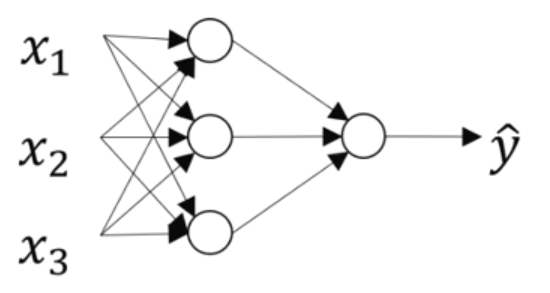
\includegraphics[width=8cm]{images/twolayers.png}
\centering
\end{figure}
Steps: 
\begin{enumerate}
	\item $z\lay{1} = W\lay{1}x + b\lay{1}$
	\item $a\lay{1} = \sigma(z\lay{1})$
	\item $z\lay{2} = W\lay{2}a\lay{2} + b\lay{2}$
	\item $a\lay{2} = \sigma(z\lay{2})$
	\item $\yhat = a\lay{2}$
	\item $L(a\lay{2}, y)$ 
\end{enumerate}
%\newpage
\subsection{Neural Network Representations}
\begin{figure}[h]
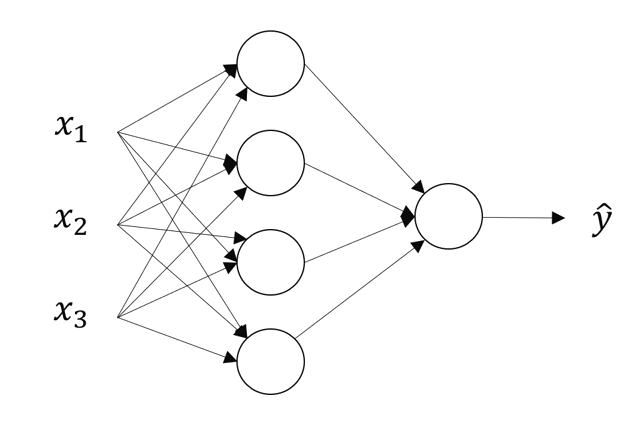
\includegraphics[width=8cm]{images/representation.png}
\centering
\end{figure}
\begin{itemize}
	\item Two layers, no. of layers = no. of hidden layers + 1 output layer
	\item $$a\lay{1} = 
	\begin{bmatrix}
		a\lay{1}_1\\
		a\lay{1}_2\\
		a\lay{1}_3\\
		a\lay{1}_4
	\end{bmatrix}
	$$
	\item $$w\lay{1}_{4\times 3}, b\lay{1}_{4\times 1}$$
	\item $$w\lay{2}_{1\times 4}, b\lay{2}_{1\times 1}$$
\end{itemize}
\begin{figure}[h]
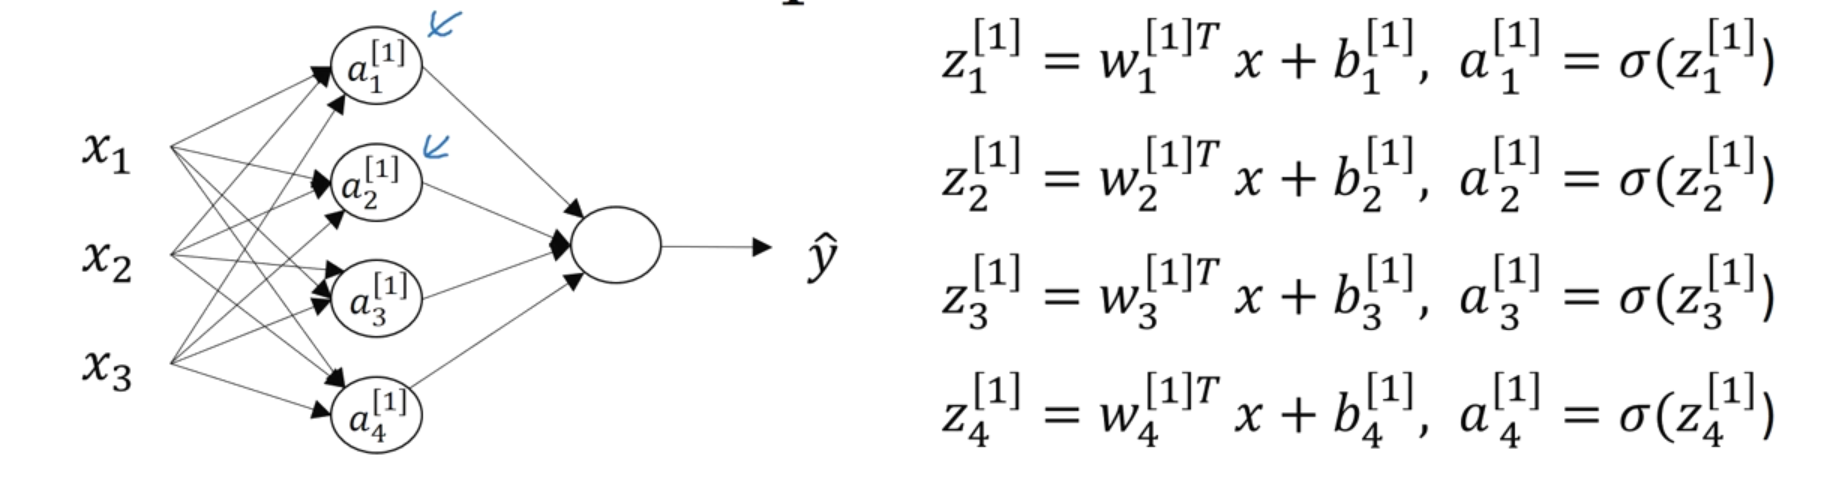
\includegraphics[scale=0.2]{images/representation2.png}
\centering
\end{figure}
$$
z\lay{1} = W\lay{1}x+b\lay{1} = \begin{bmatrix}
- w_1^{[1]T} -\\
- w_2^{[1]T} -\\
- w_3^{[1]T} -\\
- w_4^{[1]T} -
\end{bmatrix}
\begin{bmatrix}
x_1 \\
x_2 \\
x_3
\end{bmatrix} +
\begin{bmatrix}
b_1\lay{1}\\
b_2\lay{1}\\
b_3\lay{1}\\
b_4\lay{1}
\end{bmatrix}=
\begin{bmatrix}
w_1^{[1]T}x+b_1\lay{1}\\
w_2^{[1]T}x+b_2\lay{1}\\
w_3^{[1]T}x+b_3\lay{1}\\
w_4^{[1]T}x+b_4\lay{1}
\end{bmatrix}
$$

Note that $w_i^{[1]T} = $ $i$'th row of the $W\lay{1}$ matrix.  
%\newpage
Given input vector $x$: 
$$
z\lay{1}_{4\times 1} = W\lay{1}_{4 \times 3}x_{3\times 1} + b\lay{1}_{4 \times 1}
$$
$$
a\lay{1}_{4\times 1} = \sigma(z\lay{1})
$$
$$
z\lay{2}_{1\times 1} = W\lay{2}_{1\times 4}a\lay{1}_{4\times 1} + b\lay{2}_{1\times 1}
$$
$$
a\lay{2}_{1\times 1} = \sigma(z\lay{2})
$$
\subsection{Vectorization over the Full $X$ Matrix}
$$
Z\lay{1} = W\lay{1}X + b\lay{1}
$$
$$
A\lay{1} = \sigma(Z\lay{1})
$$
$$
Z\lay{2} = W\lay{2}A\lay{1} + b\lay{2}
$$
$$
A\lay{2} = \sigma(Z\lay{2})
$$

\begin{figure}[h]
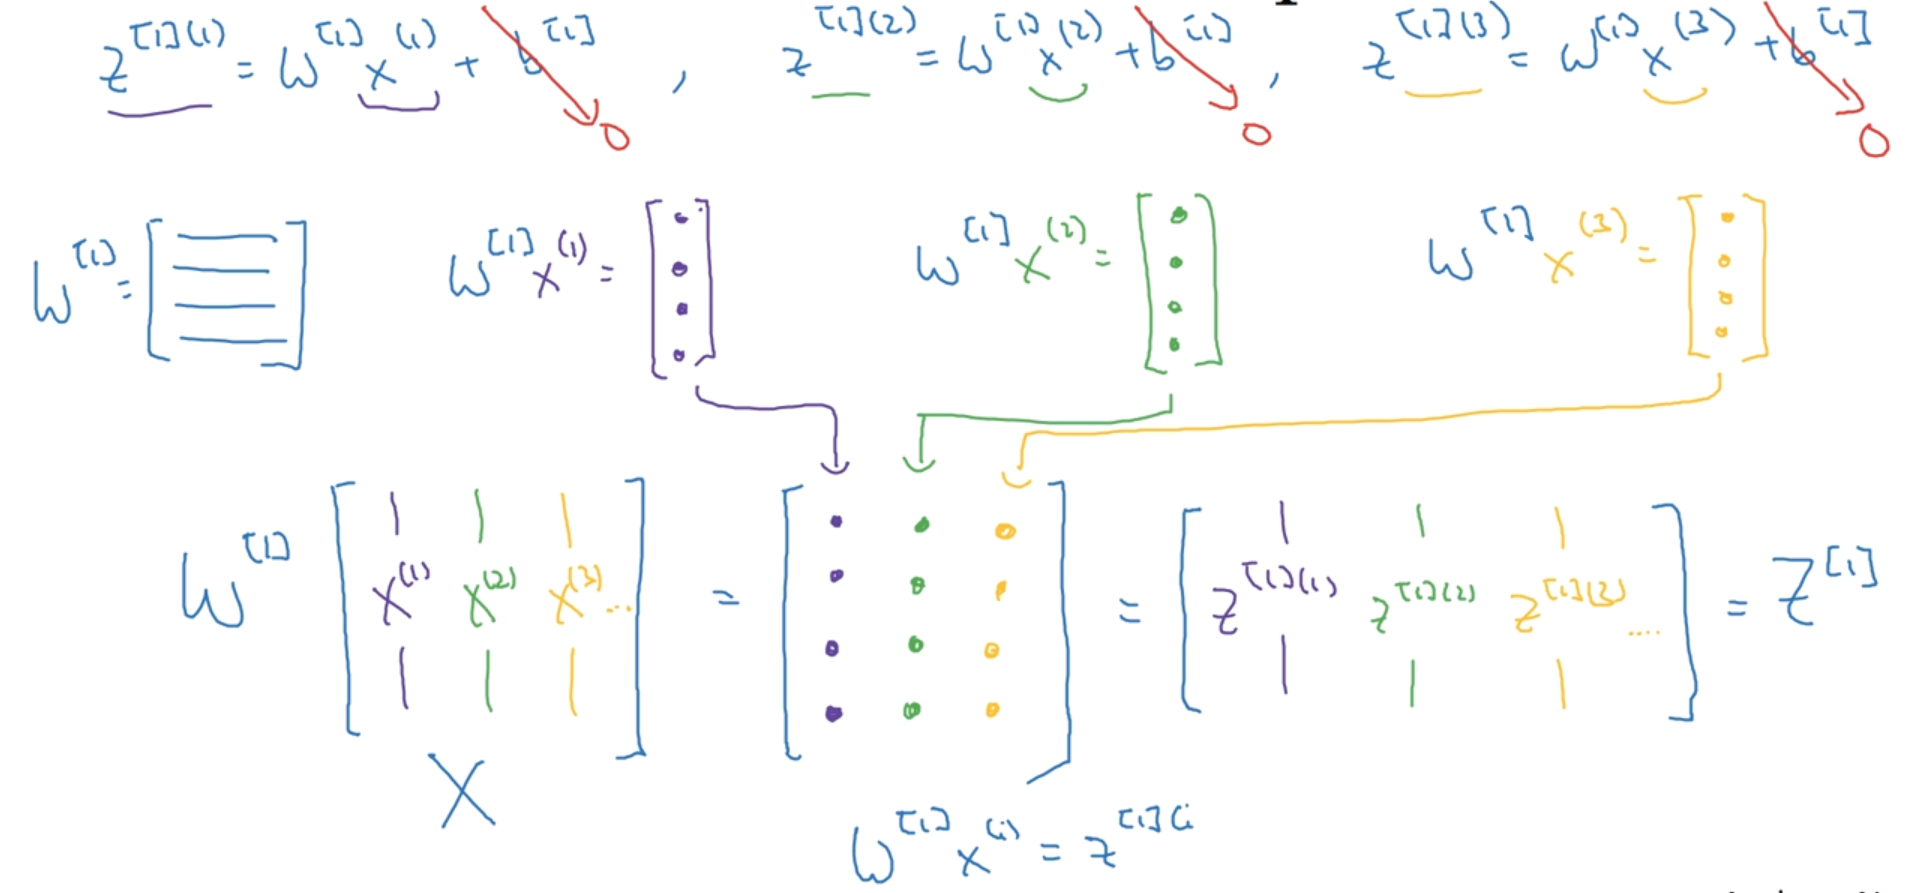
\includegraphics[scale=0.15]{images/justif.png}
\centering
\end{figure}

Where: 
$$
Z\lay{1} = \begin{bmatrix}
\vline & & \vline \\
z^{[1](1)} & \dots & z^{[1](m)}\\
\vline & & \vline \\
\end{bmatrix}
$$
$$
A\lay{1} = \begin{bmatrix}
\vline & & \vline \\
a^{[1](1)} & \dots & a^{[1](m)}\\
\vline & & \vline \\
\end{bmatrix}
$$

\subsection{Why do we need non-linear activation functions?}
Consider a identity $a=z$ activation function, which implies that $A=Z$. Given the input vector $x$: 
$$
z\lay{1}=W\lay{1}x+b\lay{1}
$$
$$
a\lay{1}=z\lay{1}
$$
$$
z\lay{2}=W\lay{2}a\lay{1}+b\lay{2}
$$
$$
a\lay{2}=z\lay{2}
$$
Let's rewrite $\yhat = a\lay{2}$ in terms of $x$: 
$$
a\lay{2} = W\lay{2}a\lay{1}+b\lay{2} = W\lay{2}\Big(W\lay{1}x+b\lay{1}\Big)+b\lay{2}
$$
$$
= W\lay{2}W\lay{1}x + W\lay{2}b\lay{1} + b\lay{2}
$$
$$
W^{'}x + b^{'}
$$
As a result, a neural network with a linear activation function is just outputting a linear combination of the input. No matter how many layer it has, it is as if they are non-existent. A linear layer is essentially useless. Using $g(z)=z$ as an activation function is allowed if you're solving a regression problem with a neural network + some other rare cases.

\subsection{Derivatives of Activation Functions}

Sigmoid: 
$$
a = g(z)=\frac{1}{1+e^{-z}}
$$ 
$$
\frac{d}{dz}g(z)=g(z)\Big(1-g(z)\Big) = a(1-a)
$$

Hyperbolic Tangent: 
$$
a= g(z) = tanh(z)
$$
$$
\frac{d}{dz}g(z)= 1-tanh^2(z)=1-a^2
$$

ReLU and Leaky ReLU: too obvious. 

\subsection{Gradient Descent for Neural Networks}
\begin{itemize}
	\item Parameters: $W\lay{1}, b\lay{1}, W\lay{2}, b\lay{2}$
	\item Parameters' Shapes: $(n\lay{1}\times n\lay{0}), (n\lay{1}\times 1), (n\lay{2}\times n\lay{1}), (n\lay{2}\times 1)$
	\item Cost Function: $J(W\lay{1}, b\lay{1}, W\lay{2}, b\lay{2}) = \frac{1}{m} \sum_{i=1}^{m}L(\yhat, y)$
\end{itemize}

Gradient Descent: 
\begin{itemize}
	\item Repeat
	\begin{itemize}
		\item[] Compute $\yhat^{(i)}$ for $i=1\dots m$
		\item[] $dW\lay{1}=\frac{\partial J}{\partial W\lay{1}}$, $db\lay{1}=\frac{\partial J}{\partial b\lay{1}}$, $dW\lay{2}=\frac{\partial J}{\partial W\lay{2}}$, $db\lay{2}=\frac{\partial J}{\partial b\lay{2}}$
		\item[] $W\lay{1} = W\lay{1} - \alpha dW\lay{1}$
		\item[] $b\lay{1} = b\lay{1} - \alpha db\lay{1}$
		\item[] $W\lay{2} = W\lay{2} - \alpha dW\lay{2}$
		\item[] $b\lay{2} = b\lay{2} - \alpha db\lay{2}$
	\end{itemize}
\end{itemize}

\begin{figure}[h]
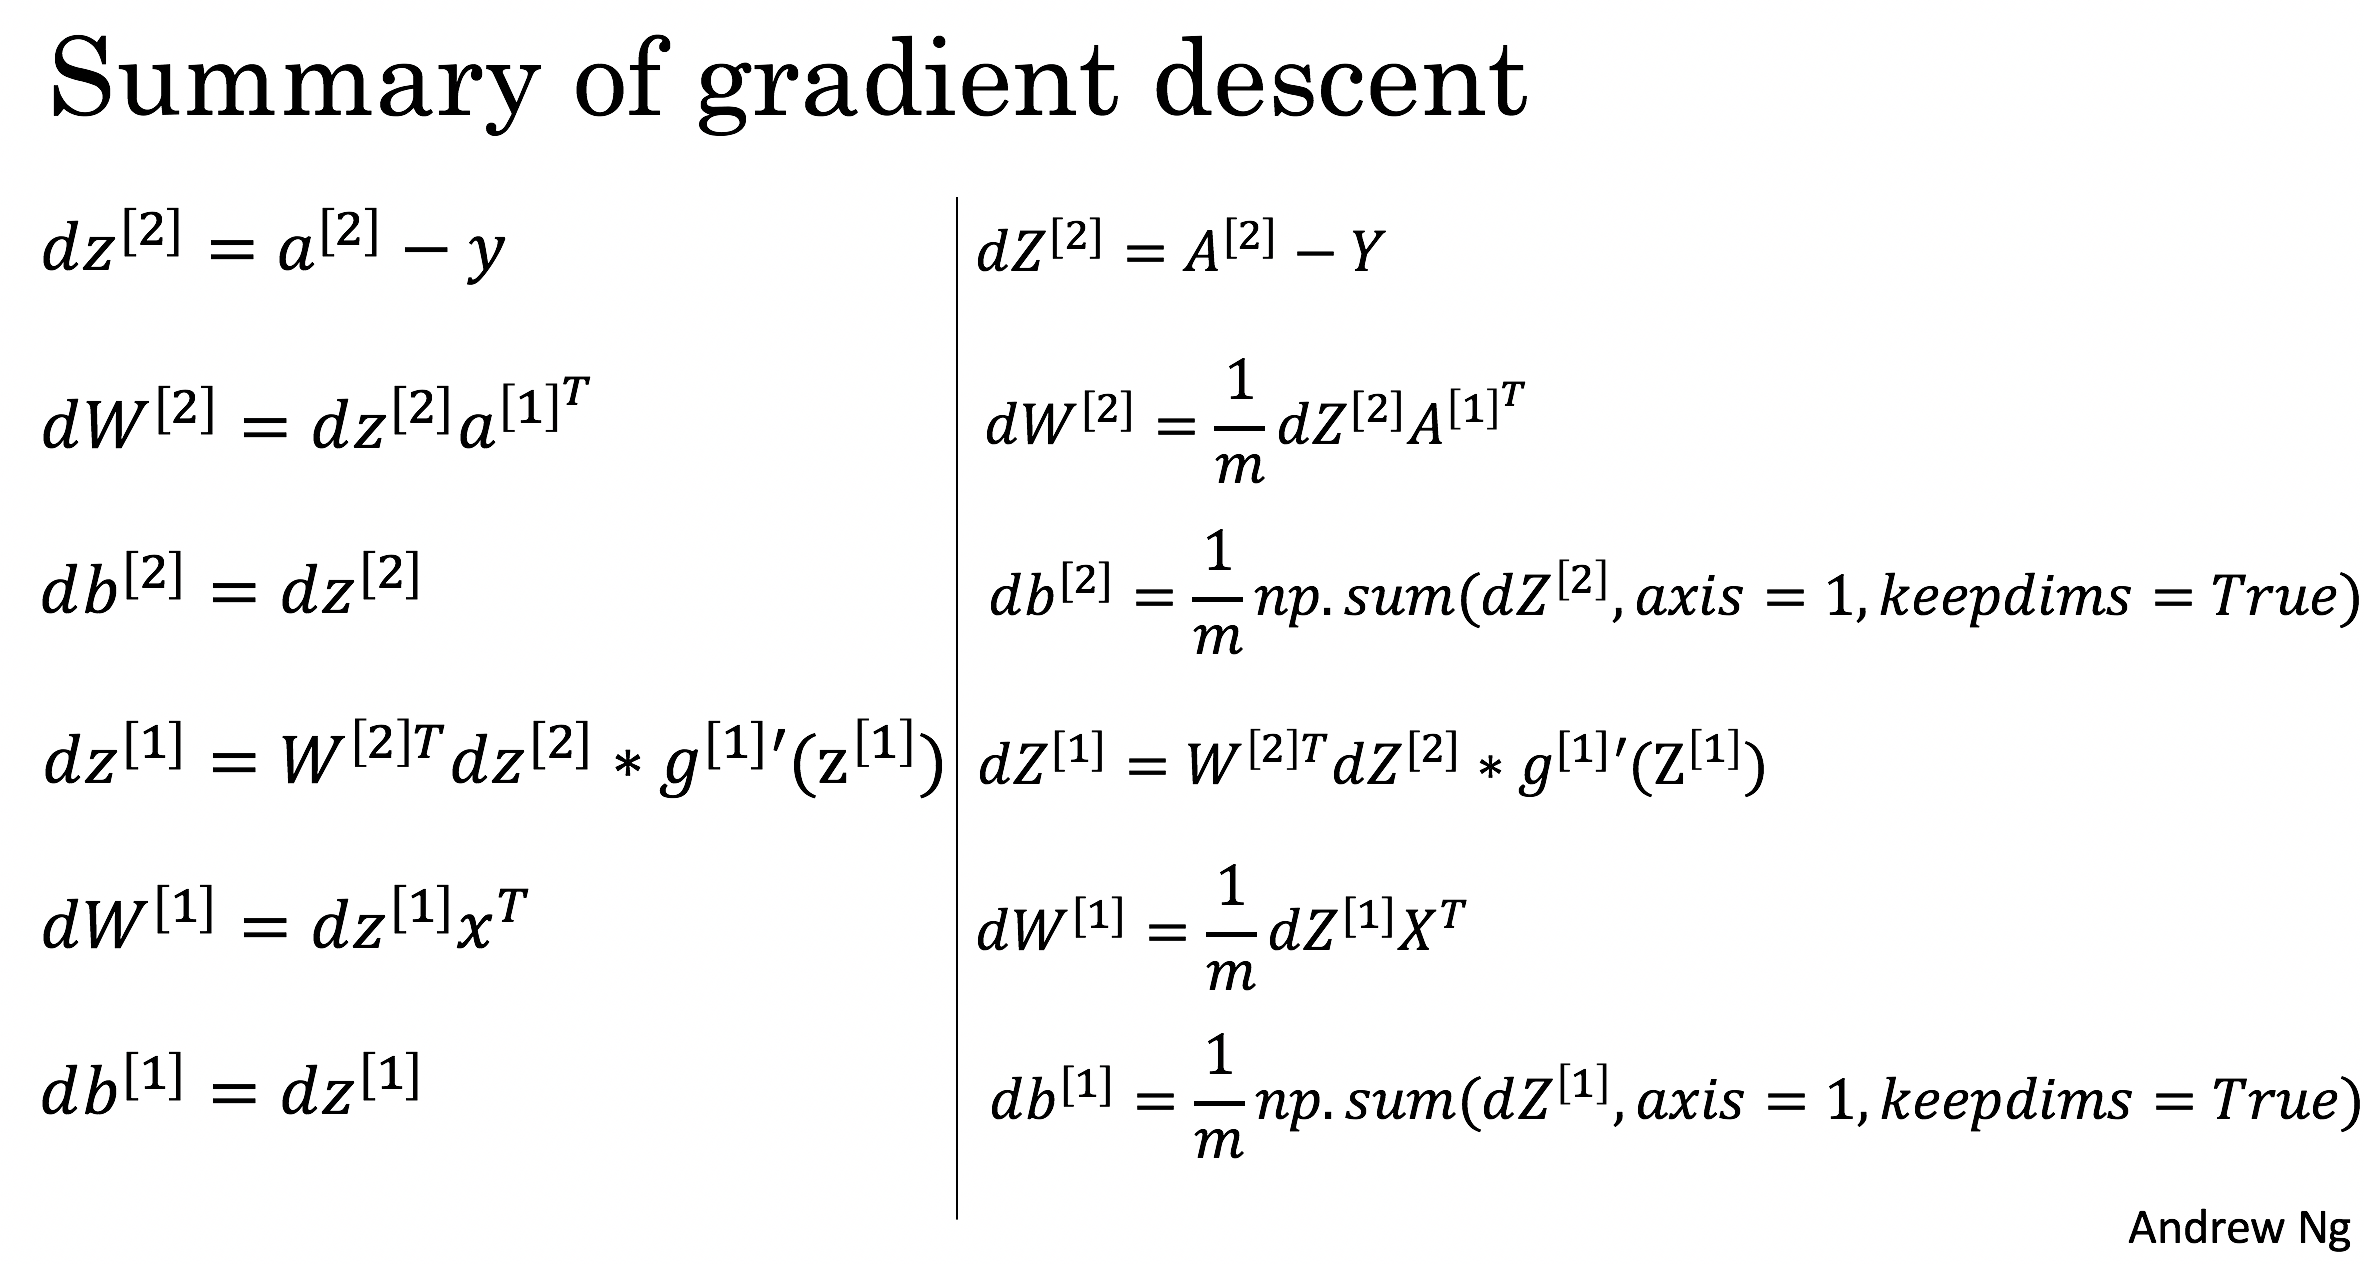
\includegraphics[scale=0.2]{images/grad_summary.png}
\centering
\end{figure}